\documentclass{article}
%%%%%%%%%%%%%%%%%%%%%%%%%%%%%%%%%%%%%%%%%%%%%%%%%%%%%%%%%%%%%%%%%%%%%%%%%%%%%%%
% PREAMBLE
%%%%%%%%%%%%%%%%%%%%%%%%%%%%%%%%%%%%%%%%%%%%%%%%%%%%%%%%%%%%%%%%%%%%%%%%%%%%%%%
\usepackage{mathtools}
\usepackage{algorithm}
\usepackage{algorithmic}
\usepackage{fancyvrb}
\usepackage{booktabs}
\usepackage{rotating}
\usepackage{tikz}
\usepackage{float}
\usepackage{hyperref}
\usepackage{subcaption}
\usetikzlibrary{arrows,decorations.pathmorphing,backgrounds,positioning,fit,matrix}
\newcommand{\DepProps}{\textsc{DepProps}}
\usepackage{titling}
\newcommand{\subtitle}[1]{%
  \posttitle{%
    \par\end{center}
    \begin{center}\large#1\end{center}
    \vskip0.5em}%
}
\begin{document}
% TITLE
\title{DM819 - Computational Geometry}
\subtitle{Fall 2015\\Project 2}
% AUTHER
\author{Mikkel Levisen and Jesper Lund}
%DATE
\maketitle
% no page number on first page
\thispagestyle{empty}
\newpage
% TABLE OF CONTENTS
\tableofcontents
% no page number on table of contents page
\thispagestyle{empty}
\newpage
% restart page number counter
\pagenumbering{arabic} 
%%%%%%%%%%%%%%%%%%%%%%%%%%%%%%%%%%%%%%%%%%%%%%%%%%%%%%%%%%%%%%%%%%%%%%%%%%%%%%%
% DOCUMENT START
%%%%%%%%%%%%%%%%%%%%%%%%%%%%%%%%%%%%%%%%%%%%%%%%%%%%%%%%%%%%%%%%%%%%%%%%%%%%%%%
\section{Introduction}
  This report details the implementation of KD-Tree and Range-Tree for 
  $n$-dimensional input. Each tree is constructed from a list of unsorted points
  and is capable of performing orthogonal range queries.
\section{KD-Tree}
\subsection{Complexity}
\section{Range-Tree}
  
\subsection{Complexity}
\section{Test}
\begin{figure}[H]
    \centering
    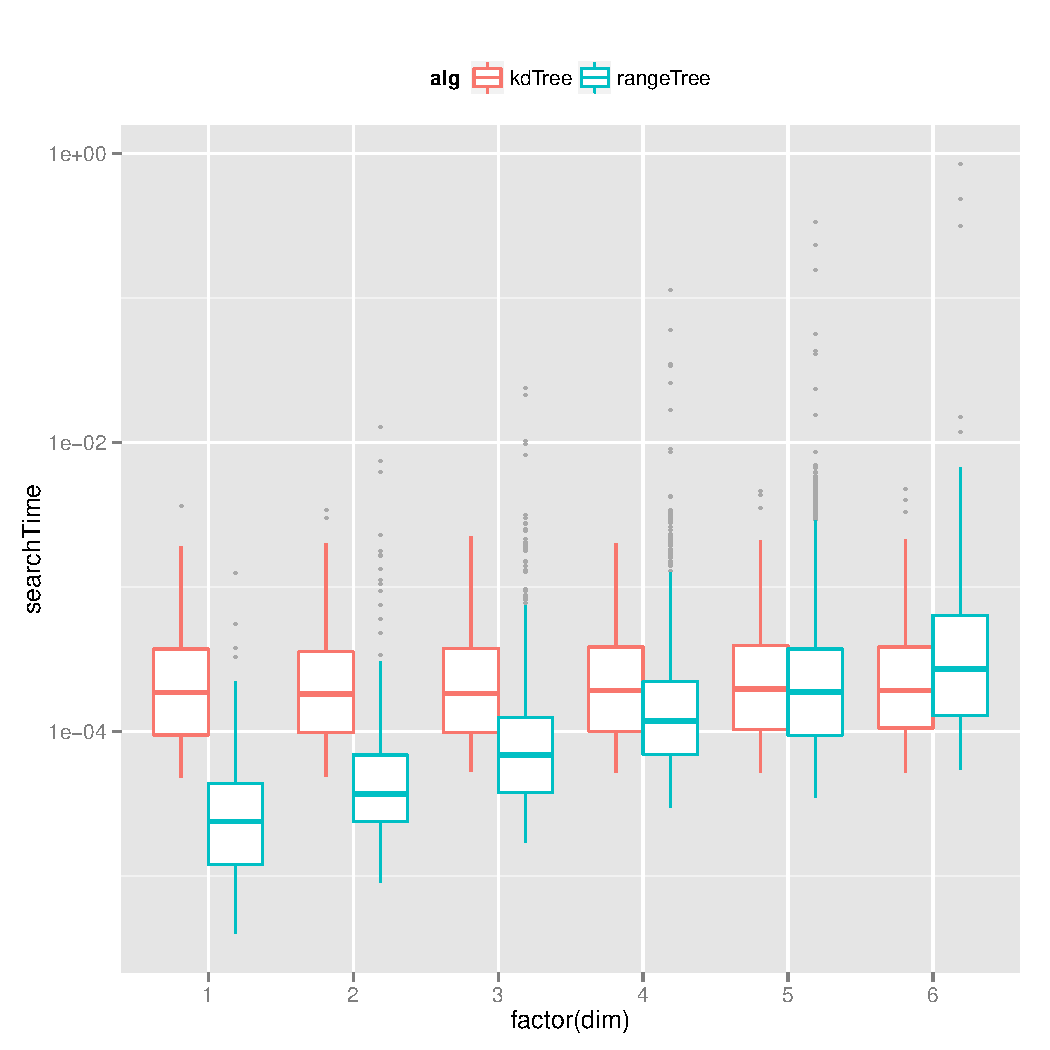
\includegraphics[width=\textwidth]{../src/R/plots/boxplot.pdf}
\end{figure}
\begin{figure}[H]
    \centering
    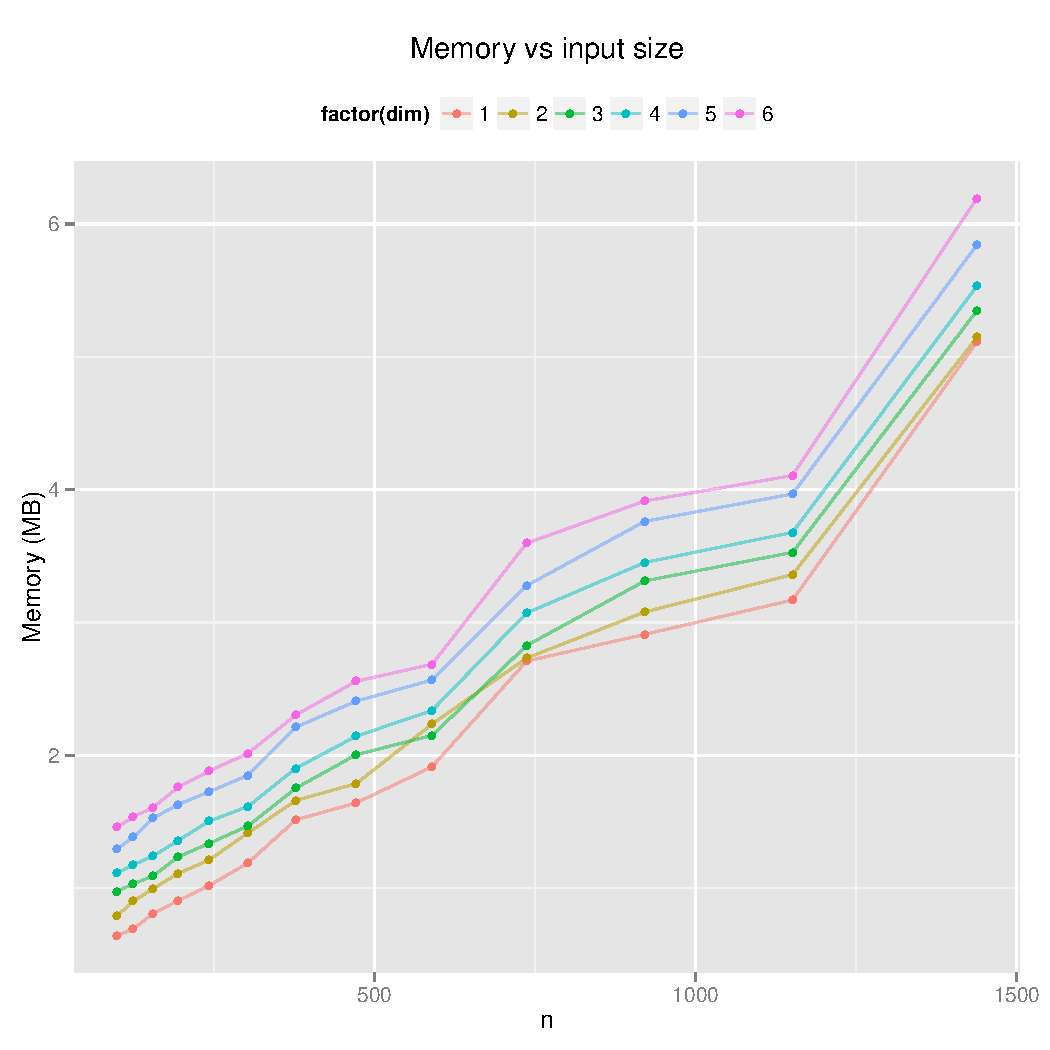
\includegraphics[width=\textwidth]{../src/R/plots/kdmem.pdf}
\end{figure}
\begin{figure}[H]
    \centering
    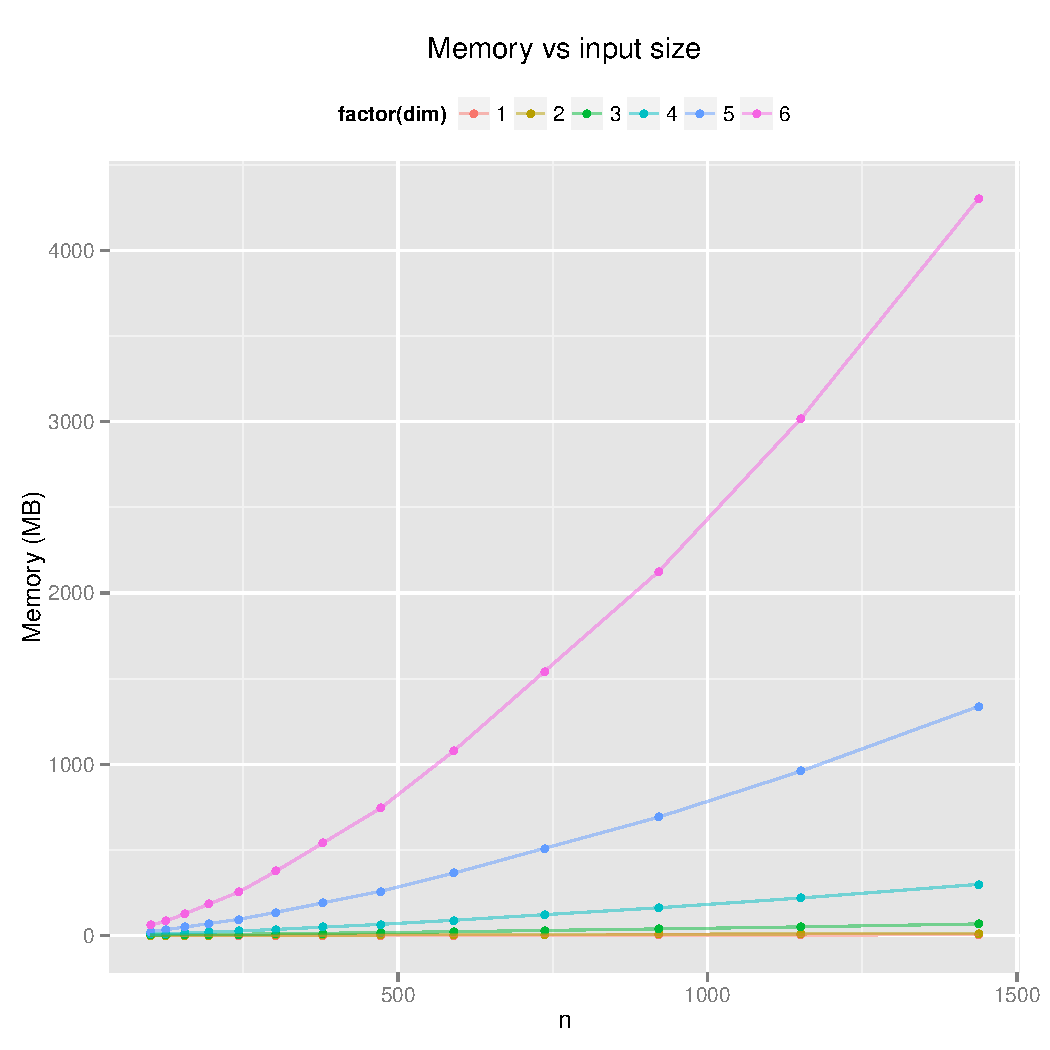
\includegraphics[width=\textwidth]{../src/R/plots/rtmem.pdf}
\end{figure}
\section{Manual}
\subsection{File Structure}
\begin{verbatim}
ROOT
|-- report/
`-- src
    |-- kdtree
    |   |-- inspect.lua
    |   |-- kdtree.lua
    |   `-- test.lua
    |-- R
    |   `-- makePlots.R
    |-- rangeTree
    |   |-- inspect.lua
    |   |-- middleclass
    |   |   `-- middleclass.lua
    |   |-- RangeTree.lua
    |   `-- test.lua
    |-- results/
    |-- runTests.py
    `-- tests
        |-- createCustomTest.lua
        |-- dimension_1/
        |-- dimension_2/
        |-- dimension_3/
        |-- dimension_4/
        |-- dimension_5/
        |-- dimension_6/
        |-- genTestSuite.lua
        `-- inspect.lua
\end{verbatim}

\section{Conclusion}
\end{document}